\documentclass{article}
\usepackage{tikz}
\usepackage{pgfplots}
\usepackage{amsmath} % Required for \begin{bmatrix}
\pgfplotsset{compat=1.18}
\usepackage{geometry}
\geometry{a4paper, margin=1cm} 

\begin{document}

\begin{center}
\section*{Visualizing Point-to-Plane (PL-ICP) Solving Steps (TikZ Series)}
\end{center}

\vspace{1cm}

% --- FIGURE 1: Initial Point Clouds & Surface Normals ---
\begin{figure}[htbp]
\centering
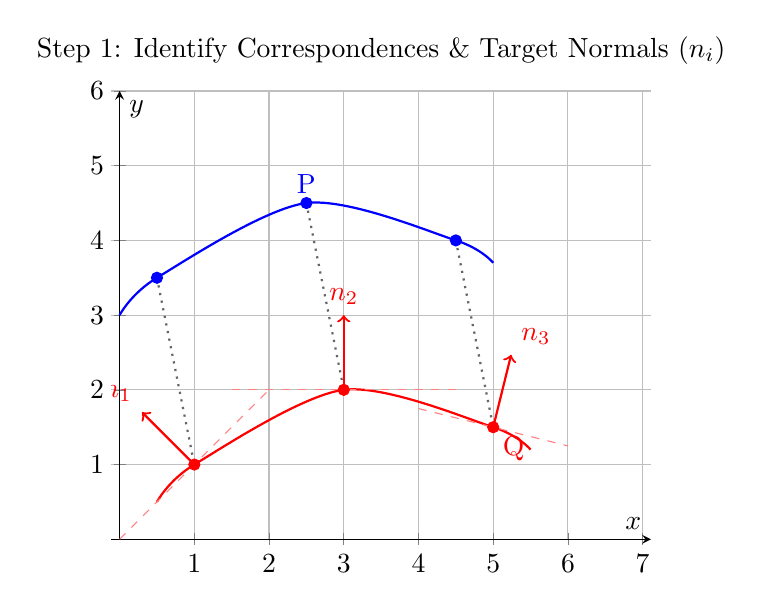
\begin{tikzpicture}
\begin{axis}[
    axis lines=middle,
    xmin=0, xmax=7, ymin=0, ymax=6,
    xtick={0, 1, ..., 7}, ytick={0, 1, ..., 6},
    axis equal, 
    xlabel=$x$, ylabel=$y$,
    title={Step 1: Identify Correspondences \& Target Normals (\(n_i\))},
    grid=both
]

% Target Point Cloud Q (red, smooth surface)
\addplot[mark=*, red, only marks, mark size=2pt] coordinates {(1,1) (3,2) (5,1.5)} node[anchor=north west] at (5,1.5) {Q};
\addplot[red, thick, smooth, mark=none] coordinates {(0.5, 0.5) (1,1) (3,2) (5,1.5) (5.5, 1.2)};

% Draw Tangent lines and Normals for Q
% q1: (1,1), tangent approx (1,1) -> normal (-1,1) normalized -> (-0.7, 0.7)
\draw[red!50!white, thin, dashed] (axis cs:0,0) -- (axis cs:2,2); 
\draw[red, ->, thick] (axis cs:1,1) -- (axis cs:0.3, 1.7) node[anchor=south east] {\(n_1\)};

% q2: (3,2), tangent horizontal -> normal (0,1)
\draw[red!50!white, thin, dashed] (axis cs:1.5,2) -- (axis cs:4.5,2);
\draw[red, ->, thick] (axis cs:3,2) -- (axis cs:3, 3) node[anchor=south] {\(n_2\)};

% q3: (5,1.5), tangent approx (1,-0.25) -> normal (0.25, 1) normalized -> (0.24, 0.97)
\draw[red!50!white, thin, dashed] (axis cs:4,1.75) -- (axis cs:6,1.25);
\draw[red, ->, thick] (axis cs:5,1.5) -- (axis cs:5.24, 2.47) node[anchor=south west] {\(n_3\)};

% Source Point Cloud P (blue, offset and rotated)
\addplot[mark=*, blue, only marks, mark size=2pt] coordinates {(0.5,3.5) (2.5,4.5) (4.5,4)} node[anchor=south] at (2.5,4.5) {P};
\addplot[blue, thick, smooth, mark=none] coordinates {(0,3) (0.5,3.5) (2.5,4.5) (4.5,4) (5,3.7)};

% Draw correspondence lines (naive nearest neighbor)
\draw[black!60!white, dotted, thick] (axis cs:0.5,3.5) -- (axis cs:1,1);
\draw[black!60!white, dotted, thick] (axis cs:2.5,4.5) -- (axis cs:3,2);
\draw[black!60!white, dotted, thick] (axis cs:4.5,4) -- (axis cs:5,1.5);

\end{axis}
\end{tikzpicture}
\caption{Step 1: Point clouds P (source) and Q (target) are matched. In PL-ICP, we must compute the local surface normal vectors \(n_i\) and tangent planes (dashed lines) for every point in the target set Q.}
\label{fig:normals}
\end{figure}

\vspace{1cm}

% --- FIGURE 2: Point-to-Point vs Point-to-Plane Error ---
\begin{figure}[htbp]
\centering
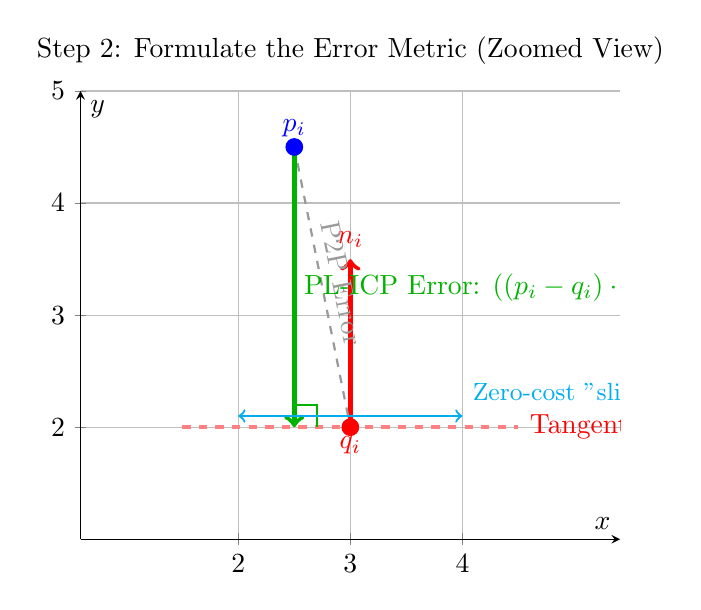
\begin{tikzpicture}
\begin{axis}[
    axis lines=middle,
    xmin=1.5, xmax=4.5, ymin=1, ymax=5,
    xtick={2, 3, 4}, ytick={2, 3, 4, 5},
    axis equal,
    xlabel=$x$, ylabel=$y$,
    title={Step 2: Formulate the Error Metric (Zoomed View)},
    grid=both
]

% Target point q2 and its tangent/normal
\addplot[mark=*, red, only marks, mark size=3pt] coordinates {(3,2)} node[anchor=north] {\(q_i\)};
\draw[red!50!white, ultra thick, dashed] (axis cs:1.5,2) -- (axis cs:4.5,2) node[anchor=west, text=red] {Tangent};
\draw[red, ->, ultra thick] (axis cs:3,2) -- (axis cs:3, 3.5) node[anchor=south] {\(n_i\)};

% Source point p2
\addplot[mark=*, blue, only marks, mark size=3pt] coordinates {(2.5,4.5)} node[anchor=south] {\(p_i\)};

% Point-to-Point Error (Hypotenuse)
\draw[black!40!white, ->, thick, dashed] (axis cs:2.5,4.5) -- (axis cs:3,2) node[midway, sloped, above] {P2P Error};

% Point-to-Plane Error (Projection onto Normal)
\draw[green!70!black, ->, ultra thick] (axis cs:2.5,4.5) -- (axis cs:2.5,2);
\draw[green!70!black, thick] (axis cs:2.5,2.2) -- (axis cs:2.7,2.2) -- (axis cs:2.7,2); % Right angle square
\node[green!70!black, anchor=west] at (axis cs:2.5, 3.25) {PL-ICP Error: \(((p_i - q_i) \cdot n_i)\)};

% Sliding visualization
\draw[cyan, <->, thick] (axis cs:2, 2.1) -- (axis cs:4, 2.1) node[anchor=south west, text=cyan, font=\small] {Zero-cost "sliding" zone};

\end{axis}
\end{tikzpicture}
\caption{Step 2: The core difference. Standard ICP penalizes the direct distance to \(q_i\) (dashed black line). PL-ICP only penalizes the perpendicular distance to the tangent plane (solid green line), allowing points to freely slide horizontally, reducing local minima.}
\label{fig:error_metric}
\end{figure}

\vspace{1cm}

% --- FIGURE 3: Linearization of Kinematics ---
\begin{figure}[htbp]
\centering
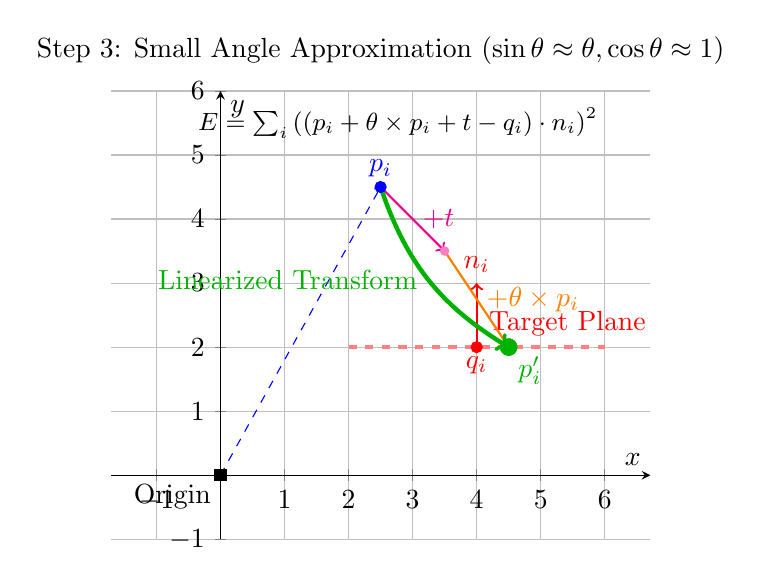
\begin{tikzpicture}
\begin{axis}[
    axis lines=middle,
    xmin=-1, xmax=6, ymin=-1, ymax=6,
    xtick={-1, 0, ..., 6}, ytick={-1, 0, ..., 6},
    axis equal,
    xlabel=$x$, ylabel=$y$,
    title={Step 3: Small Angle Approximation (\(\sin\theta \approx \theta, \cos\theta \approx 1\))},
    grid=both
]

% Origin (Center of rotation usually assumed at origin or centroid)
\addplot[mark=square*, black, only marks, mark size=2pt] coordinates {(0,0)} node[anchor=north east] {Origin};

% Target constraint
\draw[red!50!white, ultra thick, dashed] (axis cs:2,2) -- (axis cs:6,2) node[anchor=south, text=red] {Target Plane for \(p_i\)};
\addplot[mark=*, red, only marks, mark size=2pt] coordinates {(4,2)} node[anchor=north] {\(q_i\)};
\draw[red, ->, thick] (axis cs:4,2) -- (axis cs:4, 3) node[anchor=south] {\(n_i\)};

% Initial Source point
\addplot[mark=*, blue, only marks, mark size=2pt] coordinates {(2.5, 4.5)} node[anchor=south] {\(p_i\)};
\draw[blue, ->, dashed, thin] (axis cs:0,0) -- (axis cs:2.5, 4.5);

% Components of movement
% 1. Translation t
\draw[magenta, ->, thick] (axis cs:2.5, 4.5) -- (axis cs:3.5, 3.5) node[midway, right] {+\(t\)};
\addplot[mark=*, magenta!50!white, only marks, mark size=1.5pt] coordinates {(3.5, 3.5)};

% 2. Rotation component (linearized cross product: theta x p_i)
\draw[orange, ->, thick] (axis cs:3.5, 3.5) -- (axis cs:4.5, 2) node[midway, right] {+\(\theta \times p_i\)};

% Final Transformed Point
\addplot[mark=*, green!70!black, only marks, mark size=3pt] coordinates {(4.5, 2)} node[anchor=north west] {\(p_i'\)};
\draw[green!70!black, ->, ultra thick, bend right=20] (axis cs:2.5, 4.5) to node[midway, left] {Linearized Transform} (axis cs:4.5, 2);

\node[font=\small, anchor=west] at (axis cs: -0.5, 5.5) {\(E = \sum_i \left( (p_i + \theta \times p_i + t - q_i) \cdot n_i \right)^2\)};

\end{axis}
\end{tikzpicture}
\caption{Step 3: Because the rotation matrix is non-linear, we linearize the transformation by assuming the rotation angle \(\theta\) is small. The movement of \(p_i\) is decomposed into a translation vector \(t\) and a cross-product \(\theta \times p_i\). We constrain this new point \(p_i'\) to lie exactly on the target plane.}
\label{fig:linearize}
\end{figure}

\vspace{1cm}

% --- FIGURE 4: Solving the Linear System A x = b ---
\begin{figure}[htbp]
\centering
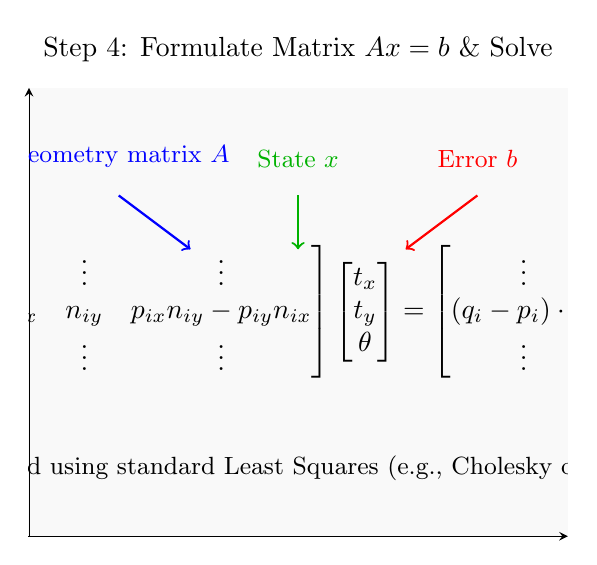
\begin{tikzpicture}
\begin{axis}[
    axis lines=middle,
    xmin=0, xmax=6, ymin=0, ymax=5,
    xtick=\empty, ytick=\empty,
    axis equal,
    xlabel=\empty, ylabel=\empty,
    title={Step 4: Formulate Matrix \(Ax=b\) \& Solve},
    grid=none,
    axis background/.style={fill=gray!5}
]

\node[anchor=center] at (axis cs:3, 2.5) {
    \( \begin{bmatrix}
    \vdots & \vdots & \vdots \\
    n_{ix} & n_{iy} & p_{ix}n_{iy} - p_{iy}n_{ix} \\
    \vdots & \vdots & \vdots
    \end{bmatrix}
    \begin{bmatrix} t_x \\ t_y \\ \theta \end{bmatrix}
    =
    \begin{bmatrix} \vdots \\ (q_i - p_i) \cdot n_i \\ \vdots \end{bmatrix} \)
};

\node[font=\small, anchor=north] at (axis cs:3, 1) {System solved using standard Least Squares (e.g., Cholesky or SVD of A)};
\node[font=\small, text=blue, anchor=south] at (axis cs:1, 4) {Geometry matrix \(A\)};
\node[font=\small, text=green!70!black, anchor=south] at (axis cs:3, 4) {State \(x\)};
\node[font=\small, text=red, anchor=south] at (axis cs:5, 4) {Error \(b\)};

\draw[->, blue, thick] (axis cs:1, 3.8) -- (axis cs:1.8, 3.2);
\draw[->, green!70!black, thick] (axis cs:3, 3.8) -- (axis cs:3, 3.2);
\draw[->, red, thick] (axis cs:5, 3.8) -- (axis cs:4.2, 3.2);

\end{axis}
\end{tikzpicture}
\caption{Step 4: Stacking the constraints from all points creates a massive over-determined linear system \(Ax=b\). Solving this yields the optimal translation components (\(t_x, t_y\)) and the rotation angle (\(\theta\)) simultaneously, bypassing the centroid calculations required in P2P-ICP.}
\label{fig:matrix}
\end{figure}

\vspace{1cm}

% --- FIGURE 5: Final Alignment (Sliding effect shown) ---
\begin{figure}[htbp]
\centering
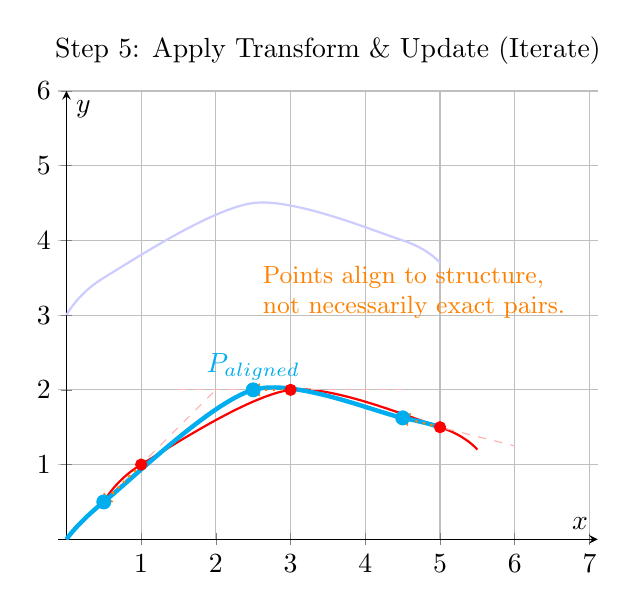
\begin{tikzpicture}
\begin{axis}[
    axis lines=middle,
    xmin=0, xmax=7, ymin=0, ymax=6,
    xtick={0, 1, ..., 7}, ytick={0, 1, ..., 6},
    axis equal, 
    xlabel=$x$, ylabel=$y$,
    title={Step 5: Apply Transform \& Update (Iterate)},
    grid=both
]

% Target Point Cloud Q (red, smooth surface)
\addplot[mark=*, red, only marks, mark size=2pt] coordinates {(1,1) (3,2) (5,1.5)};
\addplot[red, thick, smooth, mark=none] coordinates {(0.5, 0.5) (1,1) (3,2) (5,1.5) (5.5, 1.2)};

% Tangent lines representing the "plains" (faint red)
\draw[red!30!white, thin, dashed] (axis cs:0,0) -- (axis cs:2,2); 
\draw[red!30!white, thin, dashed] (axis cs:1.5,2) -- (axis cs:4.5,2);
\draw[red!30!white, thin, dashed] (axis cs:4,1.75) -- (axis cs:6,1.25);

% Original Source P (very faint)
\addplot[blue!20!white, thick, smooth, mark=none] coordinates {(0,3) (0.5,3.5) (2.5,4.5) (4.5,4) (5,3.7)};

% Transformed Source P' (cyan, snapped to tangents but NOT exactly on q_i)
\addplot[mark=*, cyan, only marks, mark size=2.5pt] coordinates {(0.5,0.5) (2.5,2) (4.5,1.625)} node[anchor=south] at (2.5,2) {\(P_{aligned}\)};
\addplot[cyan, ultra thick, smooth, mark=none] coordinates {(0,0) (0.5,0.5) (2.5,2) (4.5,1.625) (5,1.5)};

% Emphasize the slide
\draw[orange, ->, thick, dotted] (axis cs:1,1) -- (axis cs:0.5,0.5); 
\draw[orange, ->, thick, dotted] (axis cs:3,2) -- (axis cs:2.5,2); 
\draw[orange, ->, thick, dotted] (axis cs:5,1.5) -- (axis cs:4.5,1.625); 
\node[orange, font=\small, anchor=west] at (axis cs:2.5, 3.5) {Points align to structure,};
\node[orange, font=\small, anchor=west] at (axis cs:2.5, 3.1) {not necessarily exact pairs.};

\end{axis}
\end{tikzpicture}
\caption{Step 5: Visualizing the final aligned point cloud (cyan). Because the metric minimized point-to-plane distance, the cyan points map exactly onto the mathematical surfaces defined by Q's normals, but they do not need to correspond exactly to the discrete red points (\(q_i\)). This is the "sliding" characteristic of PL-ICP.}
\label{fig:final}
\end{figure}

\end{document}